%\documentclass[11pt,a4paper]{article}
\documentclass[11pt
  , a4paper
  , article
  , oneside
%  , twoside
%  , draft
]{memoir}

\usepackage{control}
\usepackage[numbers]{natbib}
\usepackage{graphicx,floatflt}

\begin{document}

\newcommand{\technumber}{
  RAON Control-Document Series\\
  Revision : v0.1,   Release : 2015.11.2}
\title{\textbf{KT Underground Laboratory Environment Monitoring System\\}}


\author{Seung Hee Nam\thanks{namsh@ibs.re.kr} \\
  Control Group \\
  Rare Isotope Science Project\\
  Institute for Basic Science\\
  Daejeon, South Korea
}

\date{\today}

\renewcommand{\maketitlehooka}{\begin{flushright}\textsf{\technumber}\end{flushright}}
%\renewcommand{\maketitlehookb}{\centering\textsf{\subtitle}}
%\renewcommand{\maketitlehookc}{C}
%\renewcommand{\maketitlehookd}{D}

\maketitle




\chapter{라즈베리파이 셋업}


KT 지하 실험실에 온습도 센서를 설치하기 전에 라즈베리 파이에 사용 할 수 있는 이미지를 생성하였다.
\begin{figure}[h]
	\begin{center}
		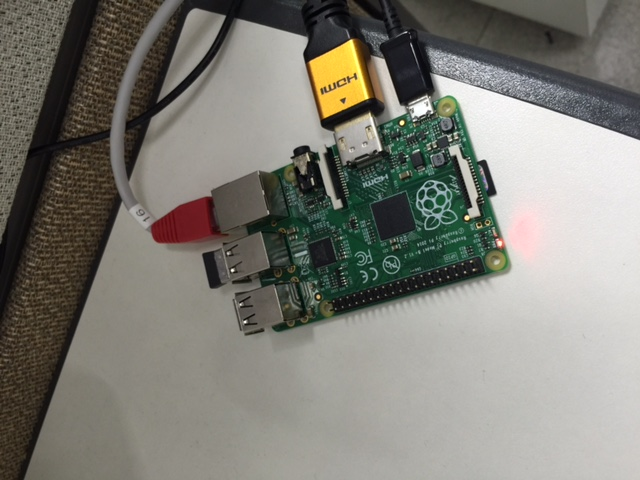
\includegraphics[width=7cm]{./images/1.JPG}
		\caption{RaspberryPi B+}
	\end{center}
\end{figure}

\subsection{Download raspbian image from}
\begin{lstlisting}[style=termstyle]
$ wget --content-disposition http://downloads.raspberrypi.org/raspbian_latest
$ unzip *raspbian*.zip
\end{lstlisting}
라즈비안을 다운받은후 압축을 풀어준다.
\subsection{Copy Image to SD Card}
\begin{lstlisting}[style=termstyle]
$ sudo dd bs=4M if=downloaded_image.img of=/dev/sdX
$ sync
$ umount /dev/sdX
\end{lstlisting}
dd를 이용해서 압축을 풀어준 라즈비안 이미지를 sd카드로 옮겨준다.\\
bs는 속도(4Mbyte)를 의미하고 if는 쓸 이미지 of는 쓰일위치이다.\\
쓰일 위치는 간단하게 df를 이용해서 확인할수있다.
\begin{lstlisting}[style=termstyle]
namsh@namsh:~/Downloads/icabu.2015.shn$ df -l
Filesystem                                              Size  Used Avail Use% Mounted on
rootfs                                                  184G   19G  156G  11% /
udev                                                     10M     0   10M   0% /dev
tmpfs                                                   1.6G  800K  1.6G   1% /run
/dev/disk/by-uuid/f4c99593-1541-478c-85df-8a2979a32cbc  184G   19G  156G  11% /
tmpfs                                                   5.0M     0  5.0M   0% /run/lock
tmpfs                                                   9.5G  185M  9.3G   2% /run/shm
/dev/sda1                                               487M  128K  486M   1% /boot/efi
/dev/sda4                                               1.6T   97G  1.5T   6% /home
\end{lstlisting}
\subsection{Insert SD Card to RaspberryPi and Expand User Partition}
PI 환경설정으로 아래와 같이 들어간후
\begin{lstlisting}[style=termstyle]
$ sudo rpi-config
\end{lstlisting}
1.Expand Filesystem을 해준뒤 리부팅 해준다.
\begin{lstlisting}[style=termstyle]
$ sudo reboot
\end{lstlisting}
\subsection{Network Configuration}
editor에는 자신이쓰는 에디터를 넣고 interfaces를 열어준다. (ex. nano, vi, emacs)
\begin{lstlisting}[style=termstyle]
$ sudo editor /etc/network/interfaces
\end{lstlisting}
쓸 ip address, netmask, gateway, dns-nameservers를 넣고 저장한다.
\begin{lstlisting}[style=termstyle]
iface eth0 inet static
address 10.1.4.206
netmask 255.255.255.0
gateway 10.1.4.254
dns-nameservers 10.1.2.240
\end{lstlisting}
무선 네트워크 설정은 다음과 같다.
\begin{lstlisting}[style=termstyle]
allow-hotplug wlan0
iface wlan0 inet static
address 10.1.4.??
netmask 255.255.255.0
gateway 10.1.4.254
dns-nameservers 10.1.2.240
wpa-scan-ssid 1
wpa-ap-ssid 1 
wpa-key-mgmt WPA-PSK
wpa-proto RSN WPA
wpa-pairwise CCMP TKIP
wpa-group CCMP TKIP
wpa-ssid "scwook"
wpa-psk "PASSWORD"
wpa-roam /etc/wpa_supplicant/wpa_supplicant.conf
iface default inet dhcp
\end{lstlisting}
pi 리부팅을 하거나 네트워크 리부팅을 해준다.
\begin{lstlisting}[style=termstyle]
$ sudo reboot
\end{lstlisting}
\begin{lstlisting}[style=termstyle]
$ sudo service network restart
\end{lstlisting}
\subsection{Package \& Firmware Upgrade}
아래와같이 패키지와 펌웨어 업데이트를 해준다.
\begin{lstlisting}[style=termstyle]
 $ sudo apt-get update
 $ sudo apt-get upgrade
 $ sudo rpi-update
\end{lstlisting}
\subsection{Setup GPIO}
라즈베리파이의 gpio를 사용하기위해서 wiringPi를 설치 해준다.
\begin{lstlisting}[style=termstyle]
 $ git clone git://git.drogon.net/wiringPi
 $ cd wiringPi
 $ sudo ./build
\end{lstlisting}
\subsection{Download and Install EPICS}
EPICS를 다운받을 위치로 이동 후 EPICS 스크립트를 다운받고 루트계정으로 접속한다.
\begin{lstlisting}[style=termstyle]
 $ git clone https://github.com/jeonghanlee/scripts_for_epics.git
 $ ~$ cd scripts_for_epics/  
 $ ~/scripts_for_epics$ sudo su
 Password: 
\end{lstlisting}
Pi에 EPICS를 설치하기위해서는 lsb\_release가 필요하므로 설치해준다.
\begin{lstlisting}[style=termstyle]
$ root@:{HOME}/scripts_for_epics# aptitude install lsb_release
\end{lstlisting}
require\_package 부터 설치한뒤 EPICS를 설치해준다.\\
설치가 끝나면 epics/R3.14.12.5/에 들어가 . setEpicsEnv를 해준다.
\begin{lstlisting}[style=termstyle]
$ root@:{HOME}/scripts_for_epics# bash require_packages.sh all
$ root@:{HOME}/scripts_for_epics# exit
$ ~/scripts_for_epics$ bash epics_default_installation.sh 
$ ~/scripts_for_epics$ cd ../epics/R3.14.12.5/
$ ~/epics/R3.14.12.5$ ls
base  extensions  setEpicsEnv.sh
$ ~/epics/R3.14.12.5$ . setEpicsEnv.sh 
\end{lstlisting}
\subsection{Download siteApp and siteLib}
아래와 같은 스크립트를 실행시켜 필요 앱과 라이브러리를 다운받는다.
\begin{lstlisting}[style=termstyle]
 $ ~/scripts_for_epics$ bash raon_cloning.sh
\end{lstlisting}
\subsection{Build an image of configured rPi and copy it to new SD casd}
dd를 이용하여 SD카드에 설치한 라즈비안과 이외의 패키지를 이미지화 시킨다.
\begin{lstlisting}[style=termstyle]
 $ sudo dd bs=4M if=name_of_new_image.img if=/dev/sd?
 $ sync
\end{lstlisting}
차후 이렇게 만든 이미지 파일은 새로운 파이를 만들때 따로 설정할 필요없이 이미지만 dd를 이용해서 옮김으로 편리하게 새로운 Pi를 만들수 있는 강점이 있다.
\begin{lstlisting}[style=termstyle]
$ sudo dd bs=4M if=/dev/sd? of=name_of_new_image.img
\end{lstlisting}
아래와같이 새로운 SD카드에 이미지를 쓰면 이전과 똑같은 Pi가 만들어진다.
\begin{lstlisting}[style=termstyle]
 $ sudo dd bs=4M if=name_of_new_image.img if=/dev/sd?
 $ sync
\end{lstlisting}
\subsection{Auto reconnection wireless LAN}
무선인터넷 사용중 무선인터넷에 끊김이 발생할때 파이는 자동으로 무선인터넷을 잡아주지 않기 때문에 다시 접속하여 사용해야한다. 이런 불편을 없애려면 아래와 같은 코드를 추가해 주어야한다.
\begin{lstlisting}[style=termstyle]
$ cd /etc/ifplugd/action.d/
$ sudo mv ifupdown ifupdown.original
$ sudo cp /etc/wpa_supplicant/ifupdown.sh ./ifupdown
$ sudo reboot
\end{lstlisting}

\chapter{모니터링 파이용 케이스 디자인}
모니터링 파이용 케이스를 만들기 위해서 스케치업 3D 툴을 이용하였고 Archiver Appliance를 이용해 온도와 습도 값을 저장하였다 그리고 통계프로그램인 R을 이용해서 온도의 오차나 경향성을 확인하고 분석했다.
\section{스케치업을 이용한 케이스 디자인}
스케치업을 통해서 디자인한 케이스는 Version1~8까지 7번의 디자인 변경이 있었고 version8은 version7 케이스의 테스트가 끝난뒤 디자인되어 현재 적용된 케이스는 version7 케이스이다.
\clearpage
\begin{center}
	\begin{figure}[h]
		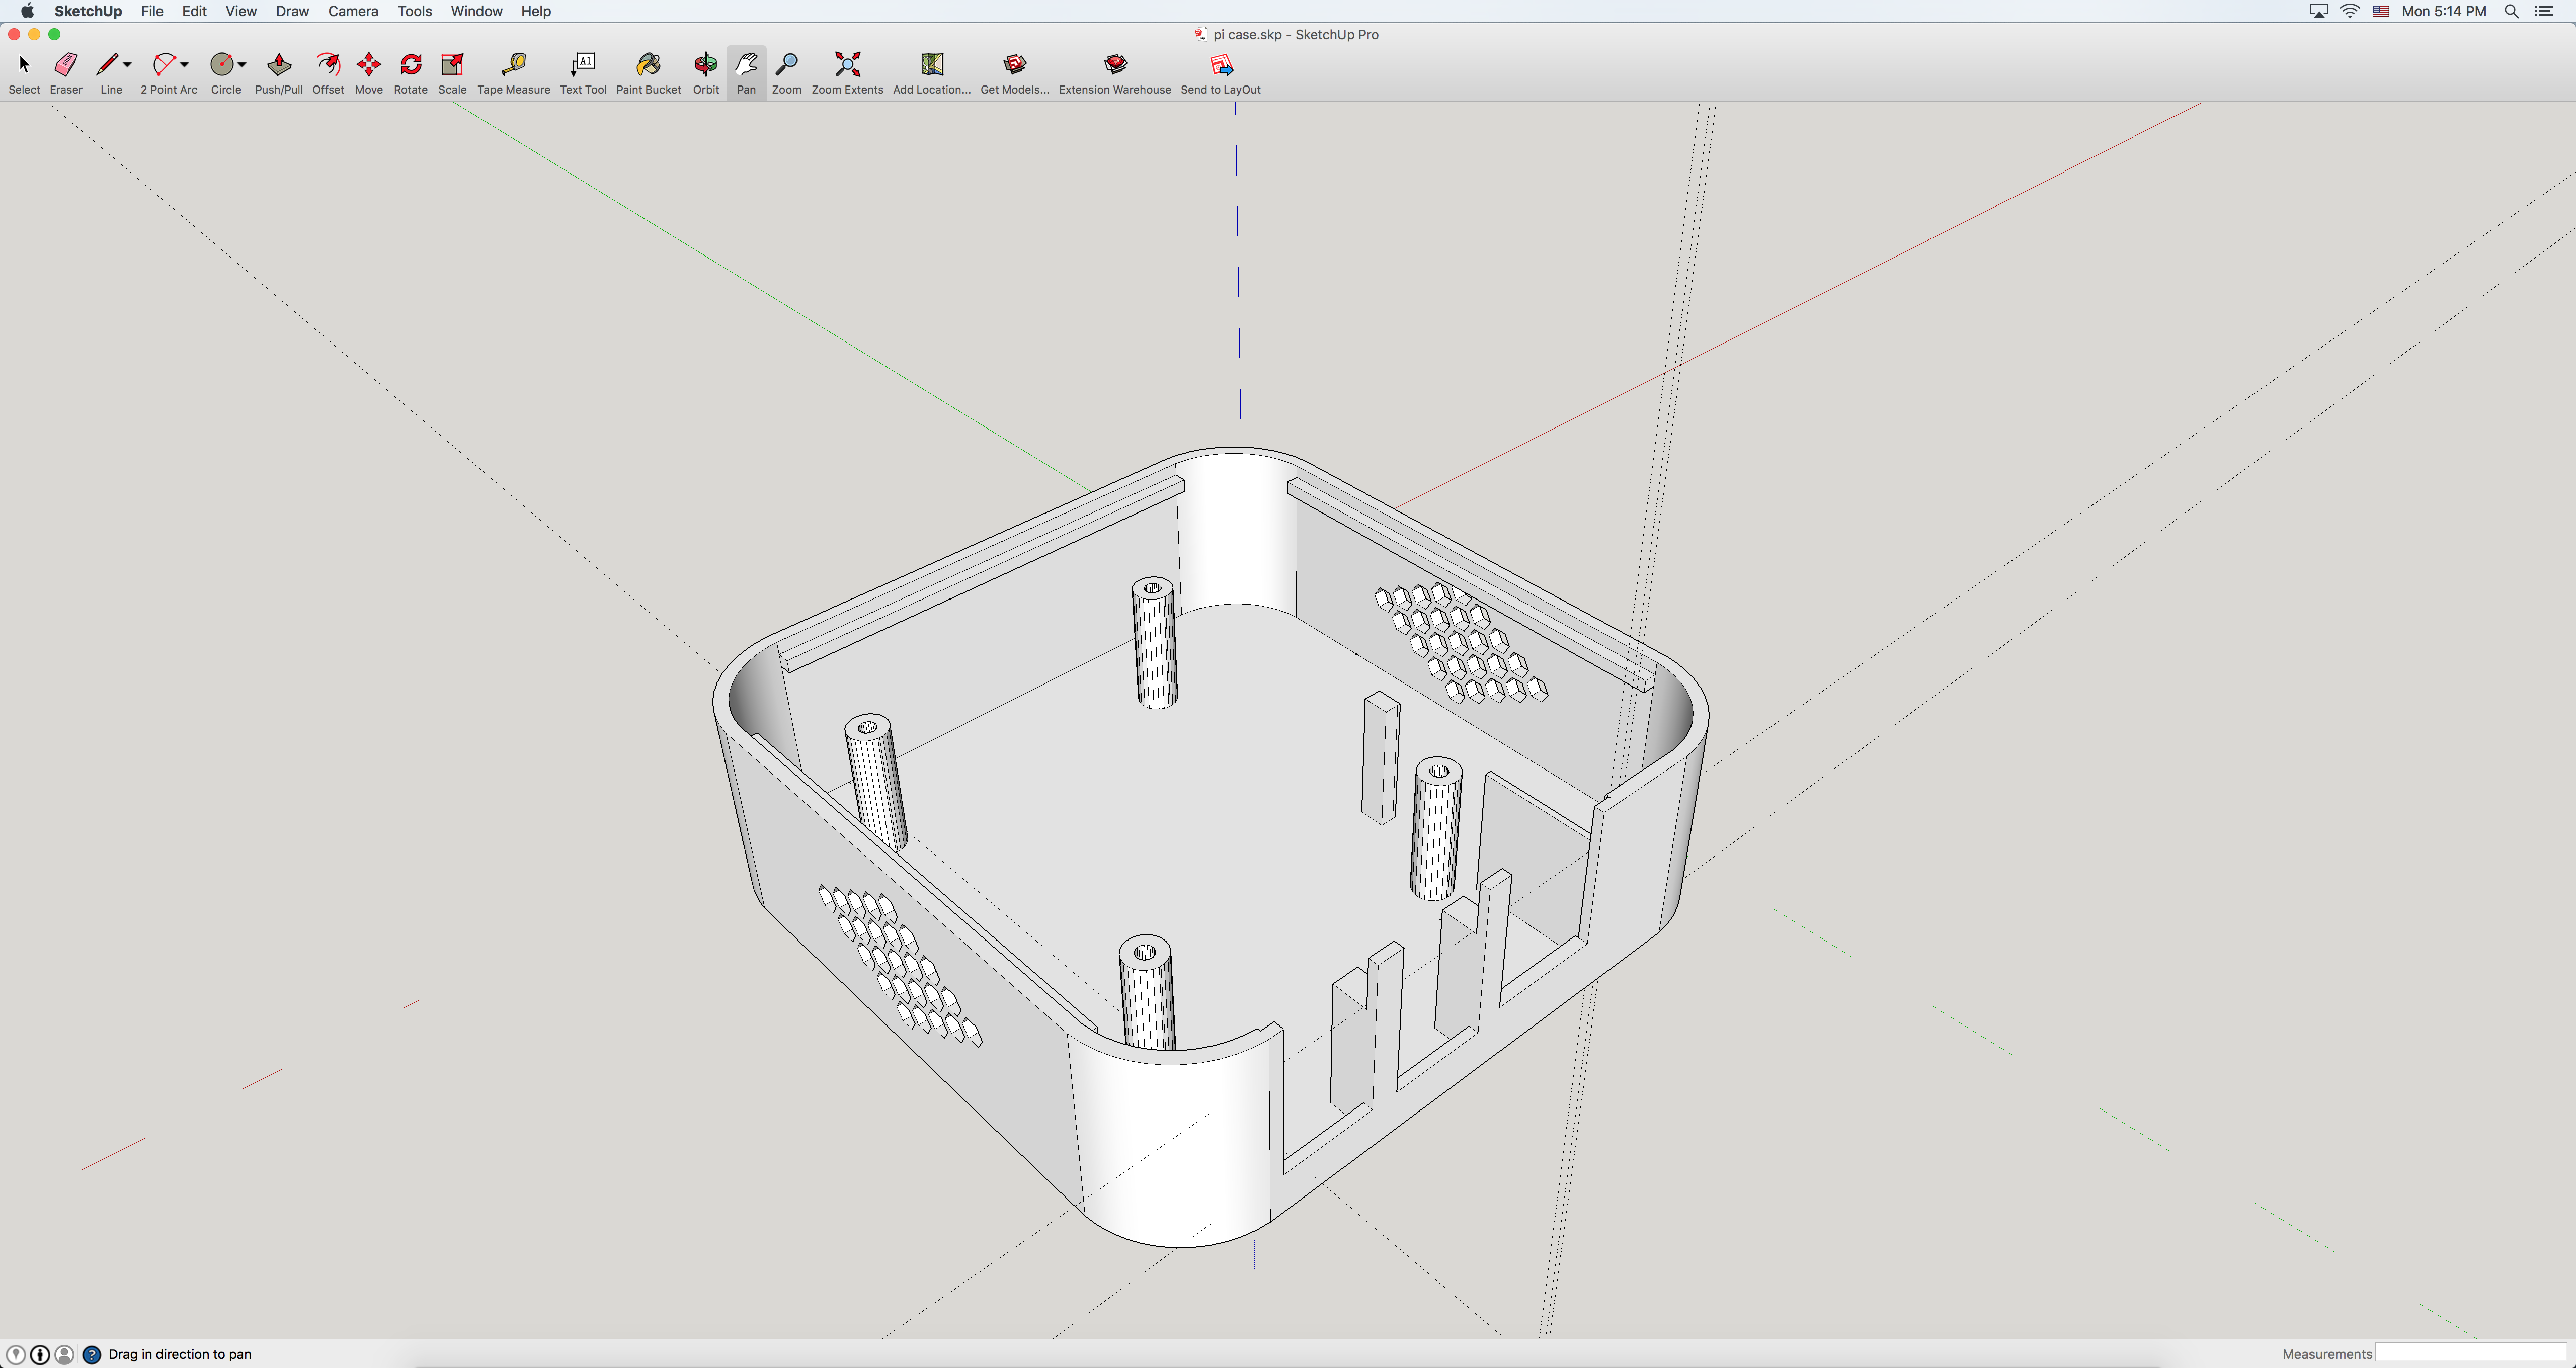
\includegraphics[width=8cm]{./images/V1.png}
		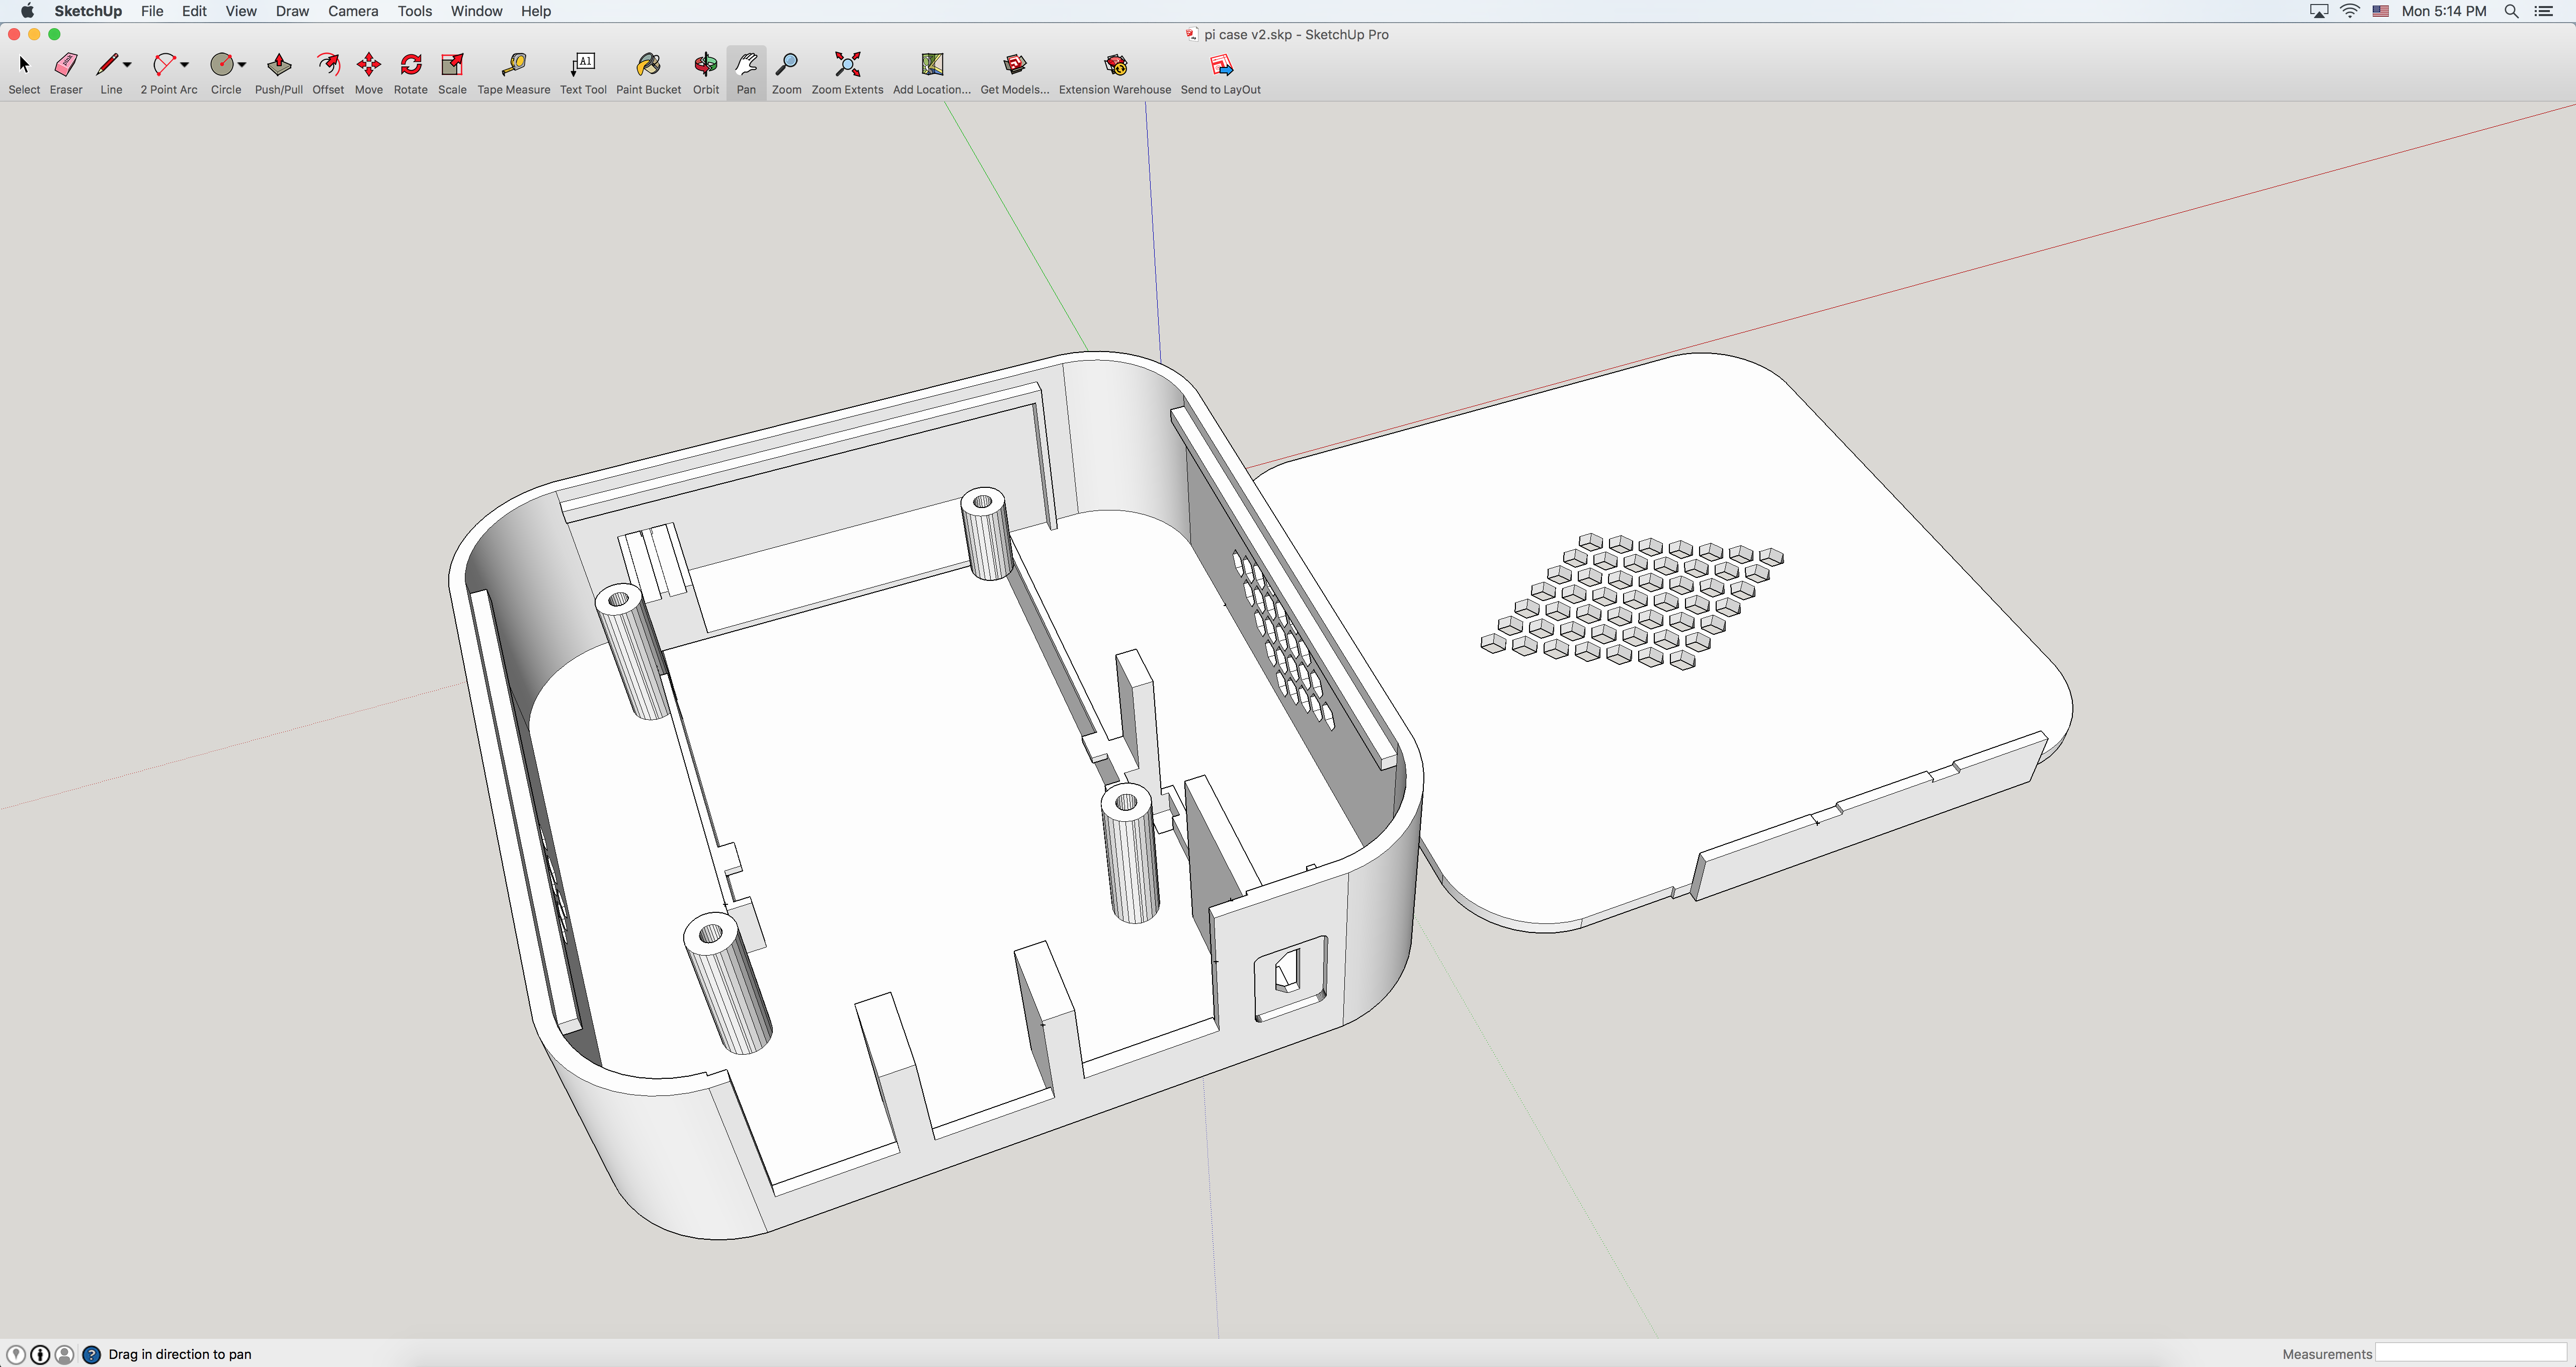
\includegraphics[width=8cm]{./images/V2.png}
		\caption{Pi Case Version1 and Version2}
	\end{figure}
\end{center}
\begin{center}
	\begin{figure}[h]
		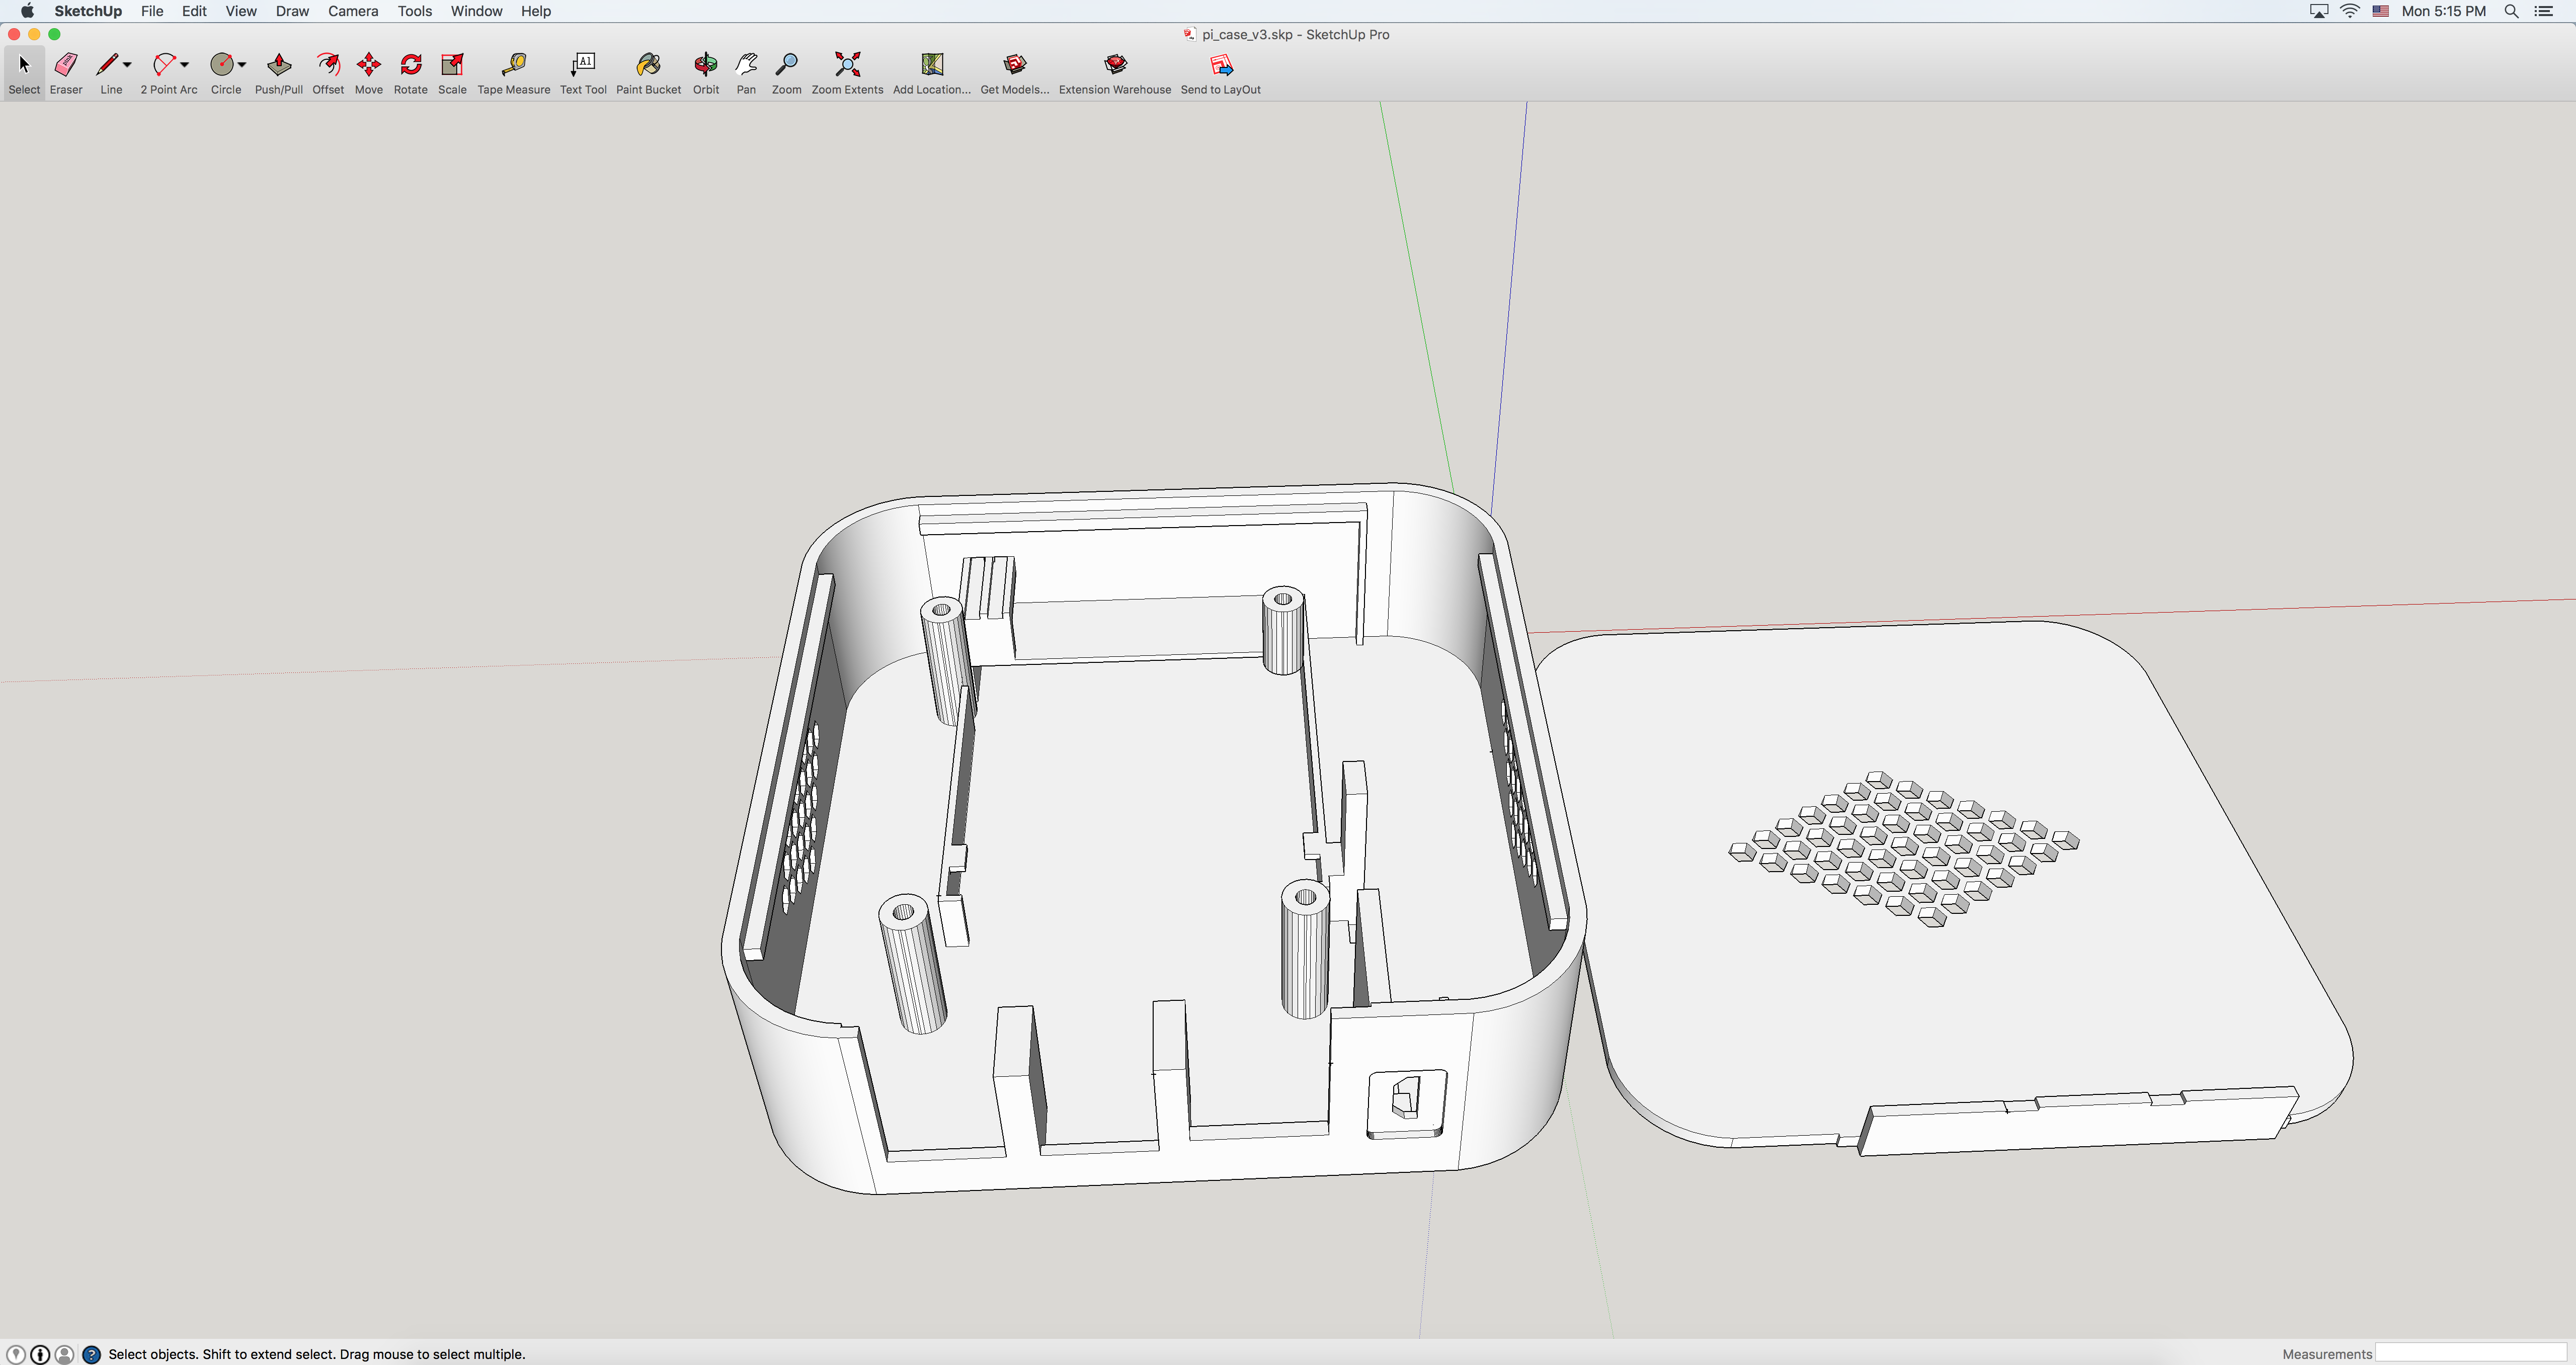
\includegraphics[width=8cm]{./images/V3.png}
		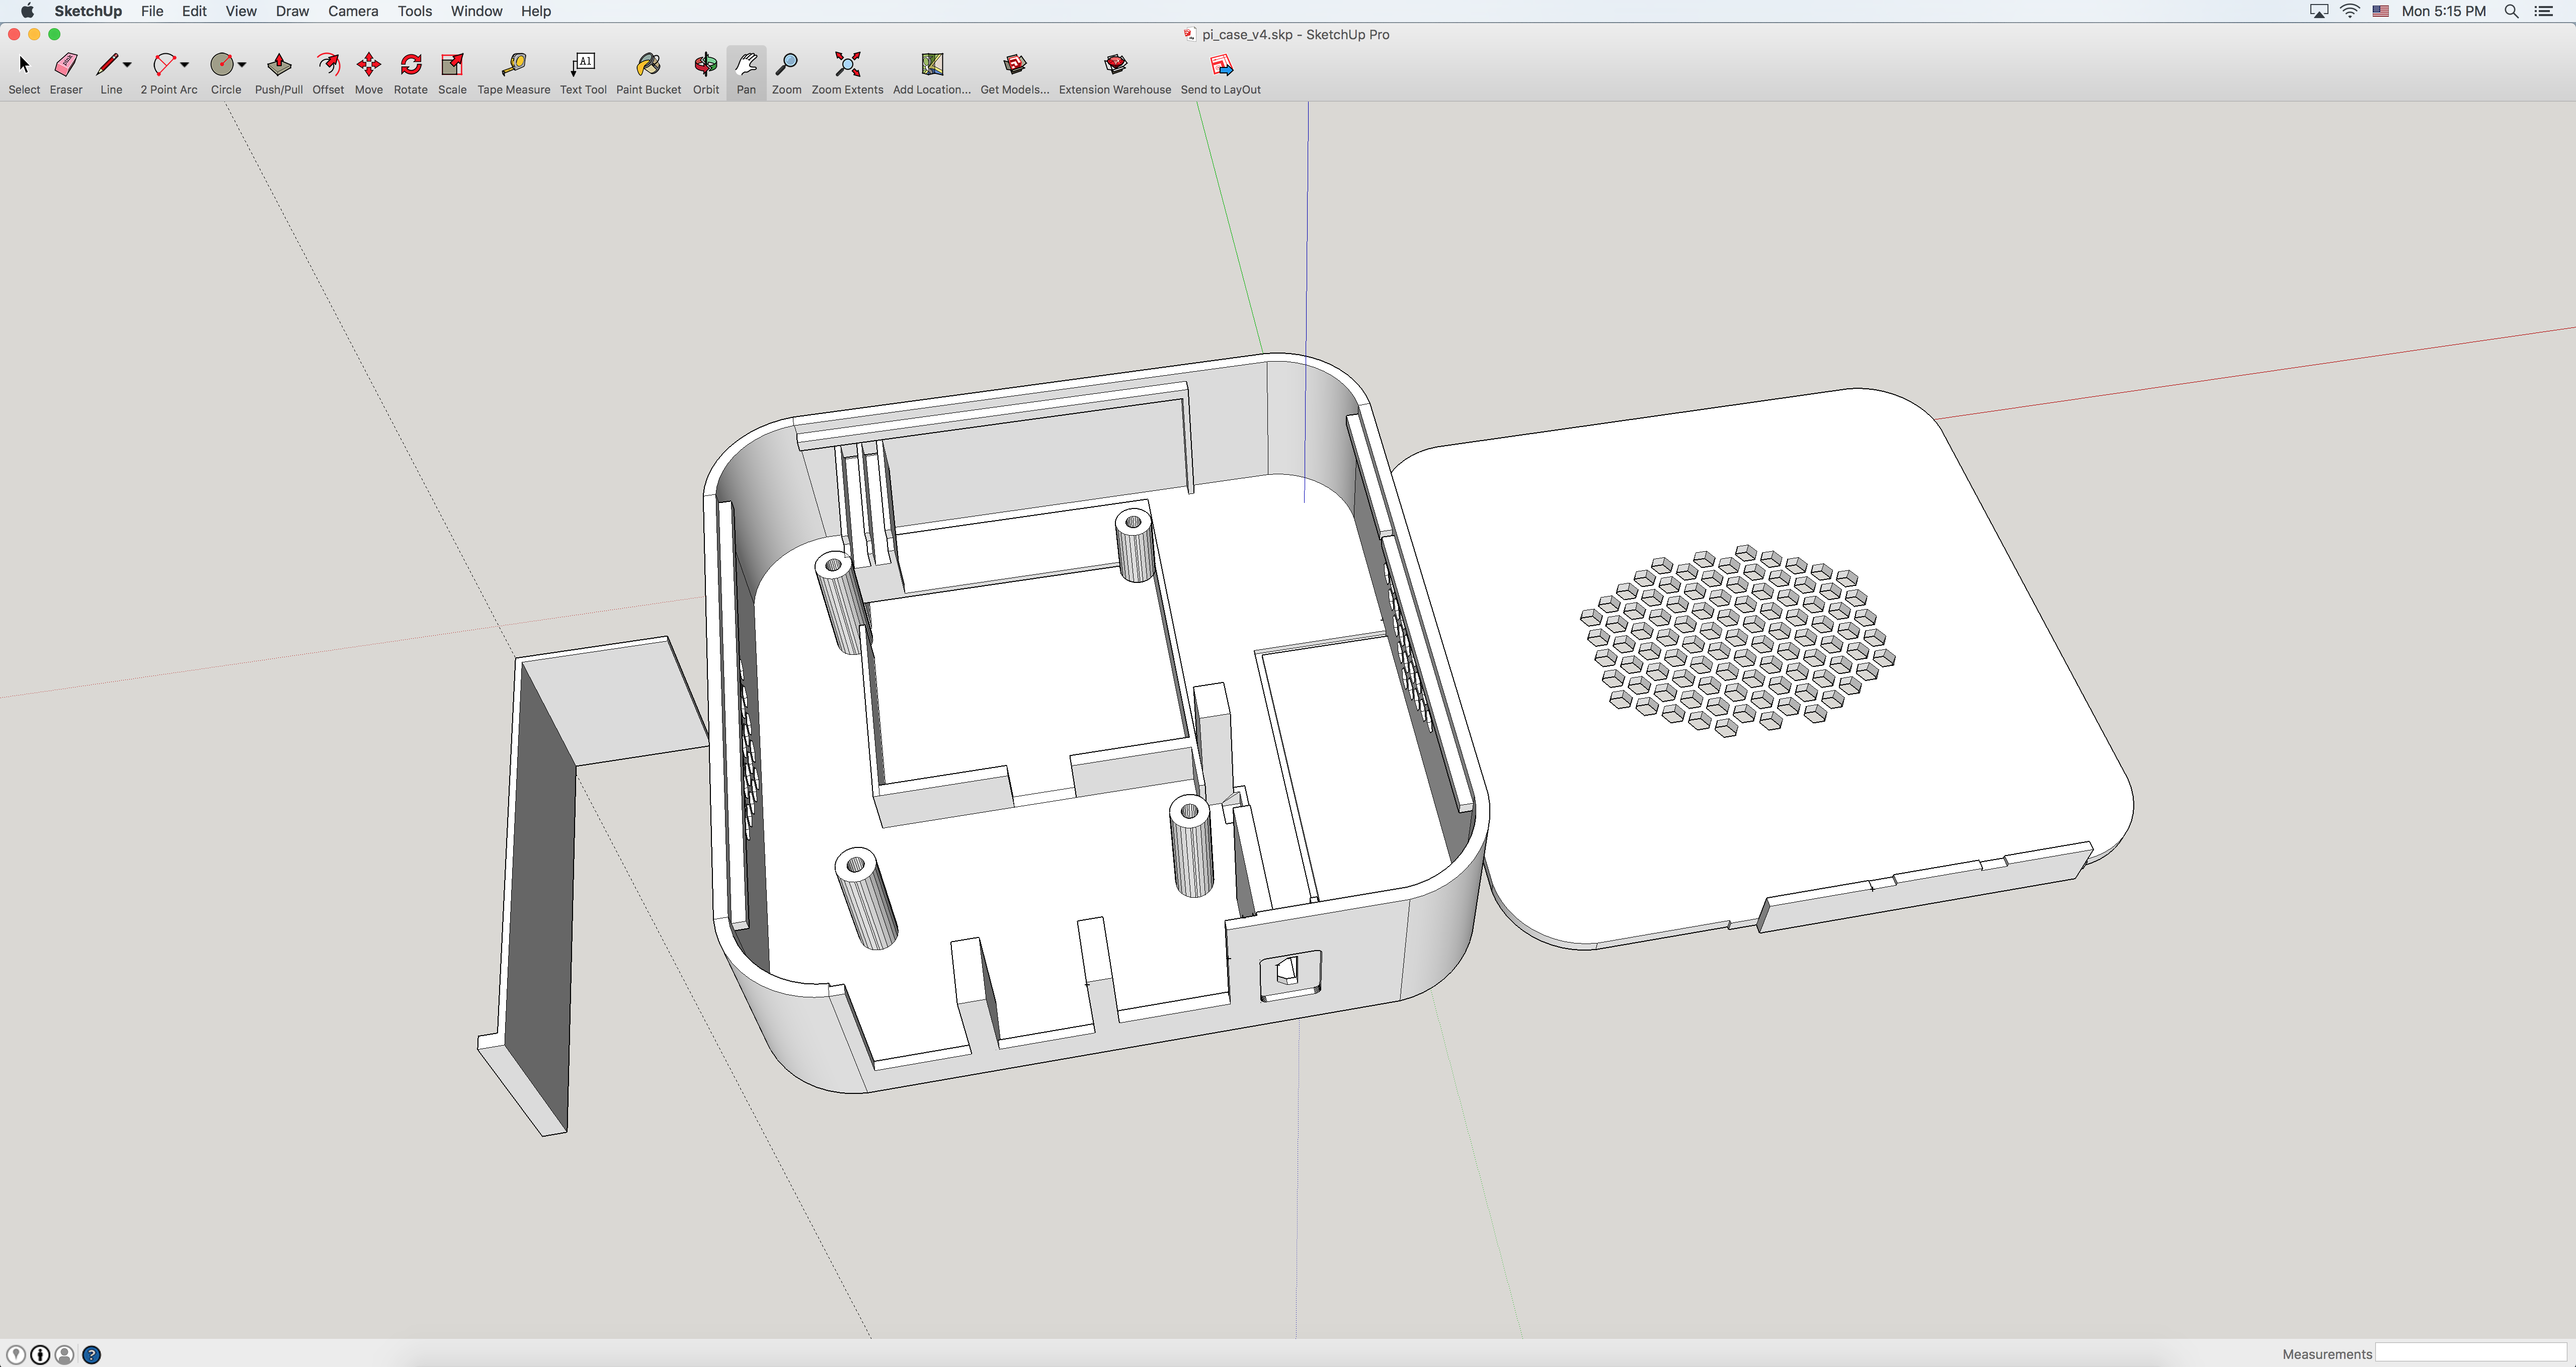
\includegraphics[width=8cm]{./images/V4.png}
		\caption{Pi Case Version3 and Version4}
	\end{figure}
\end{center}
\begin{center}
	\begin{figure}[h]
		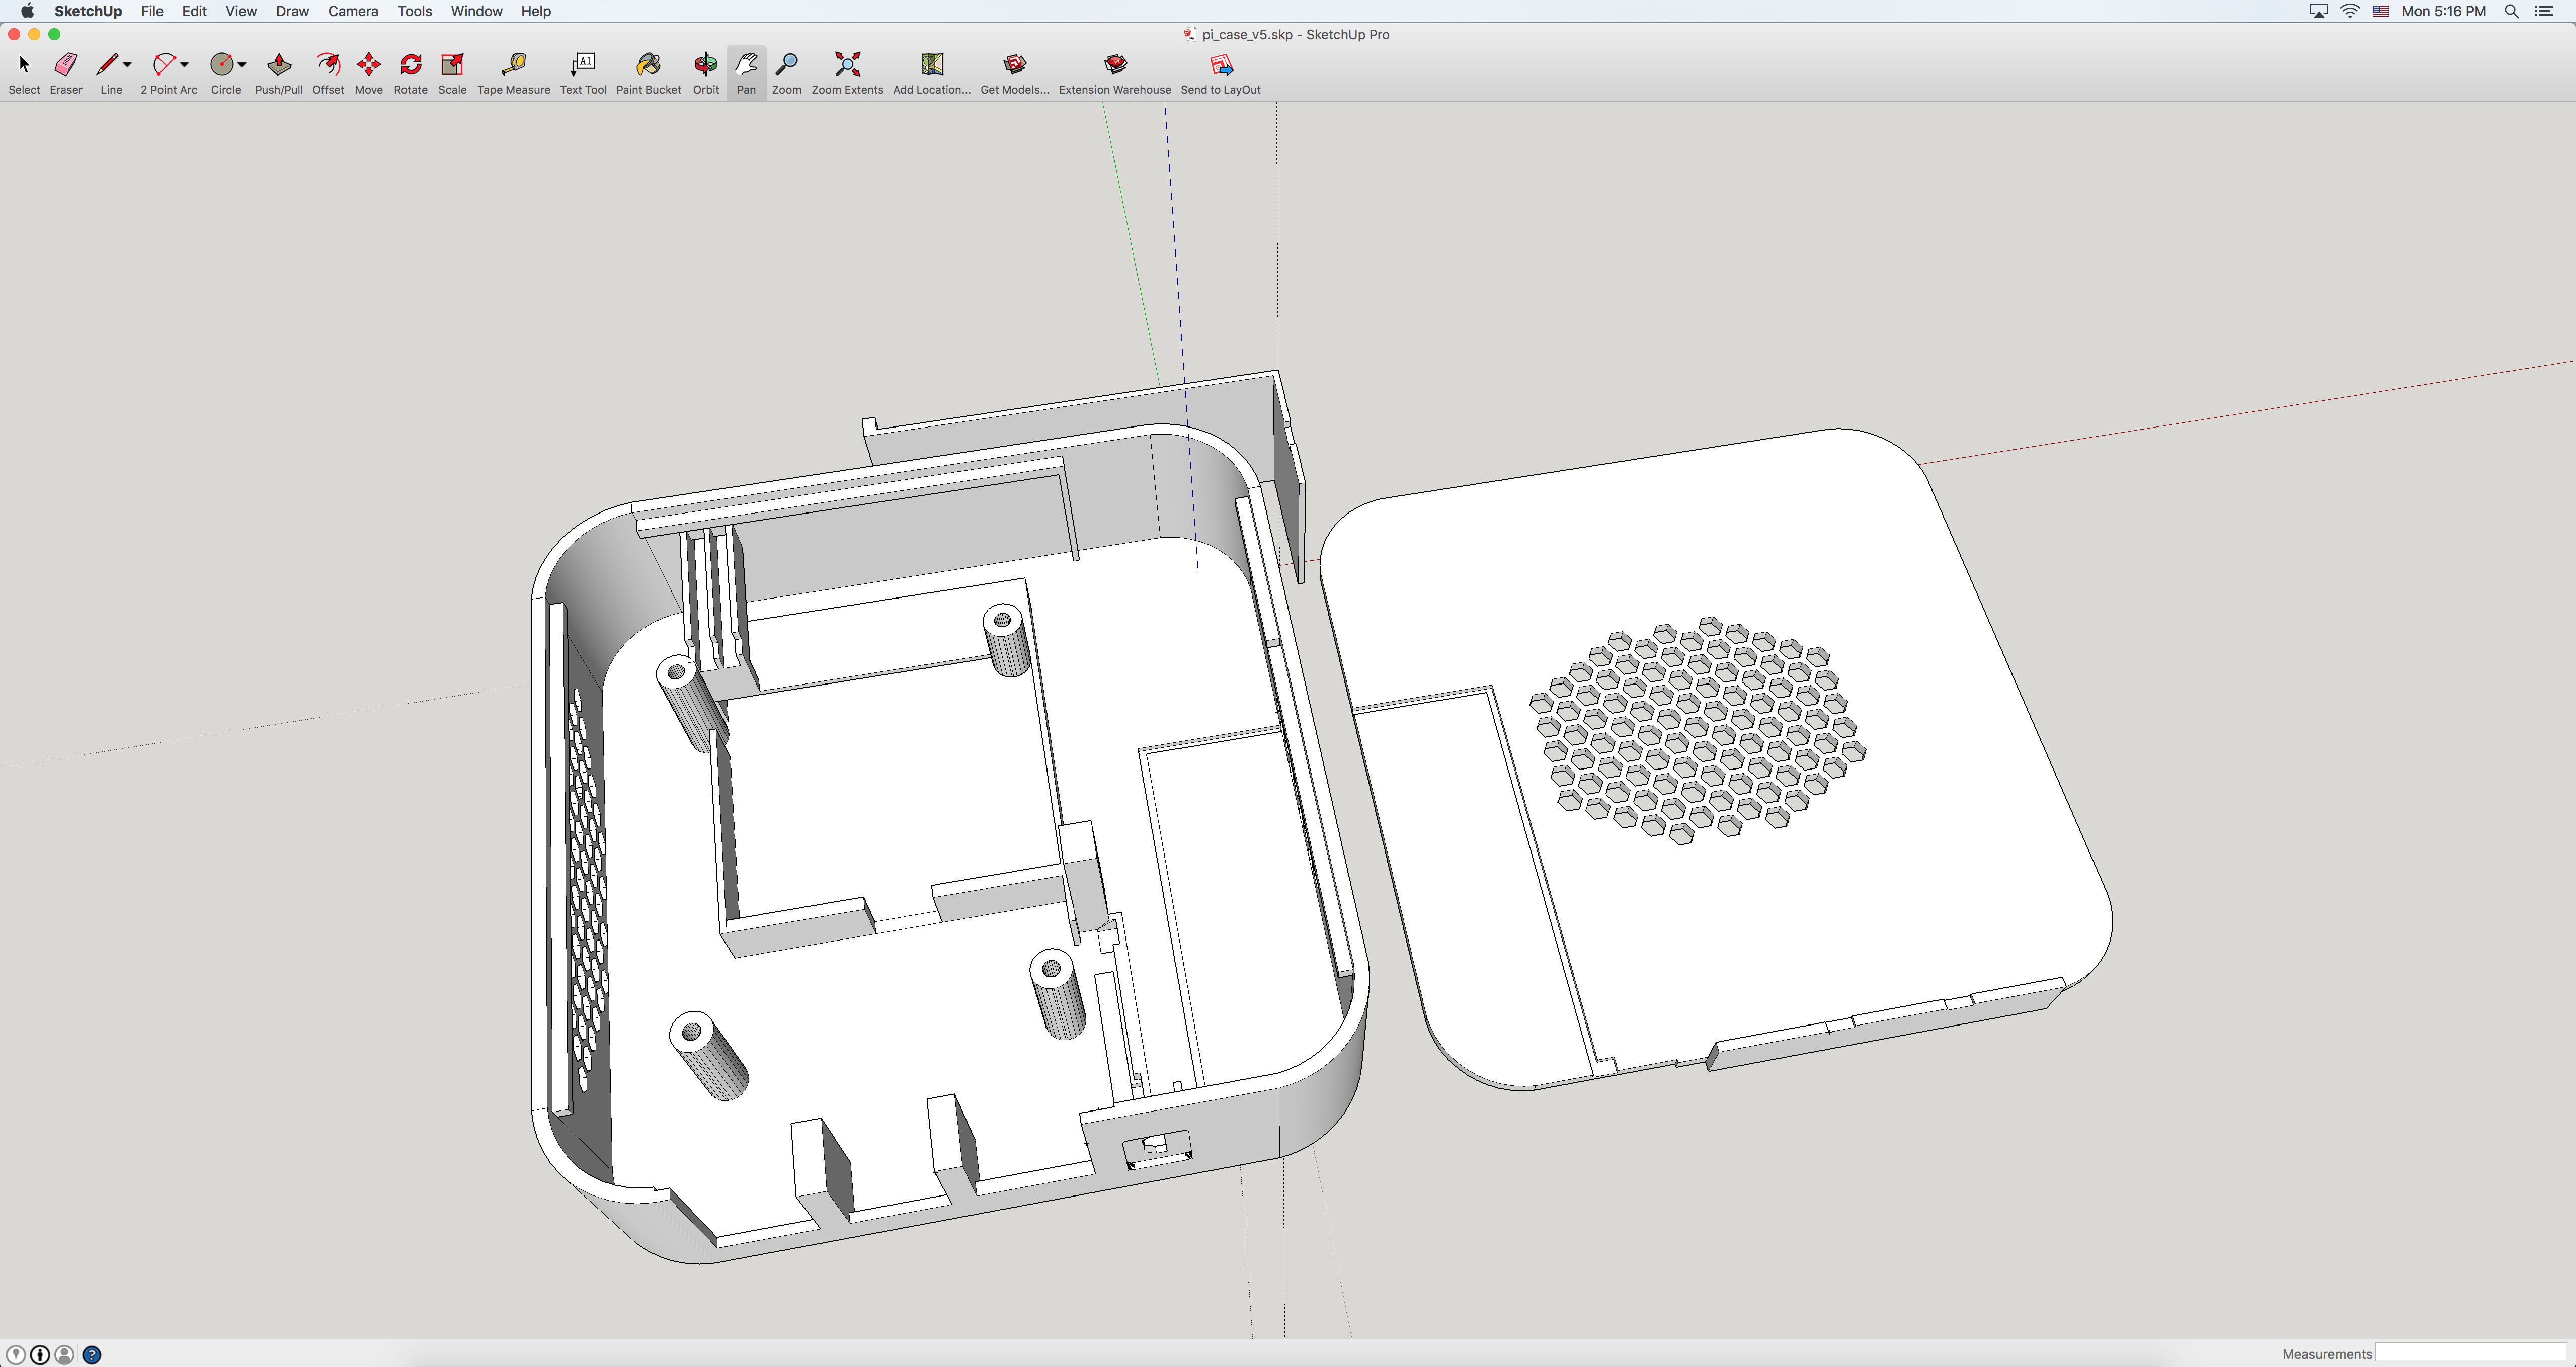
\includegraphics[width=8cm]{./images/V5.png}
		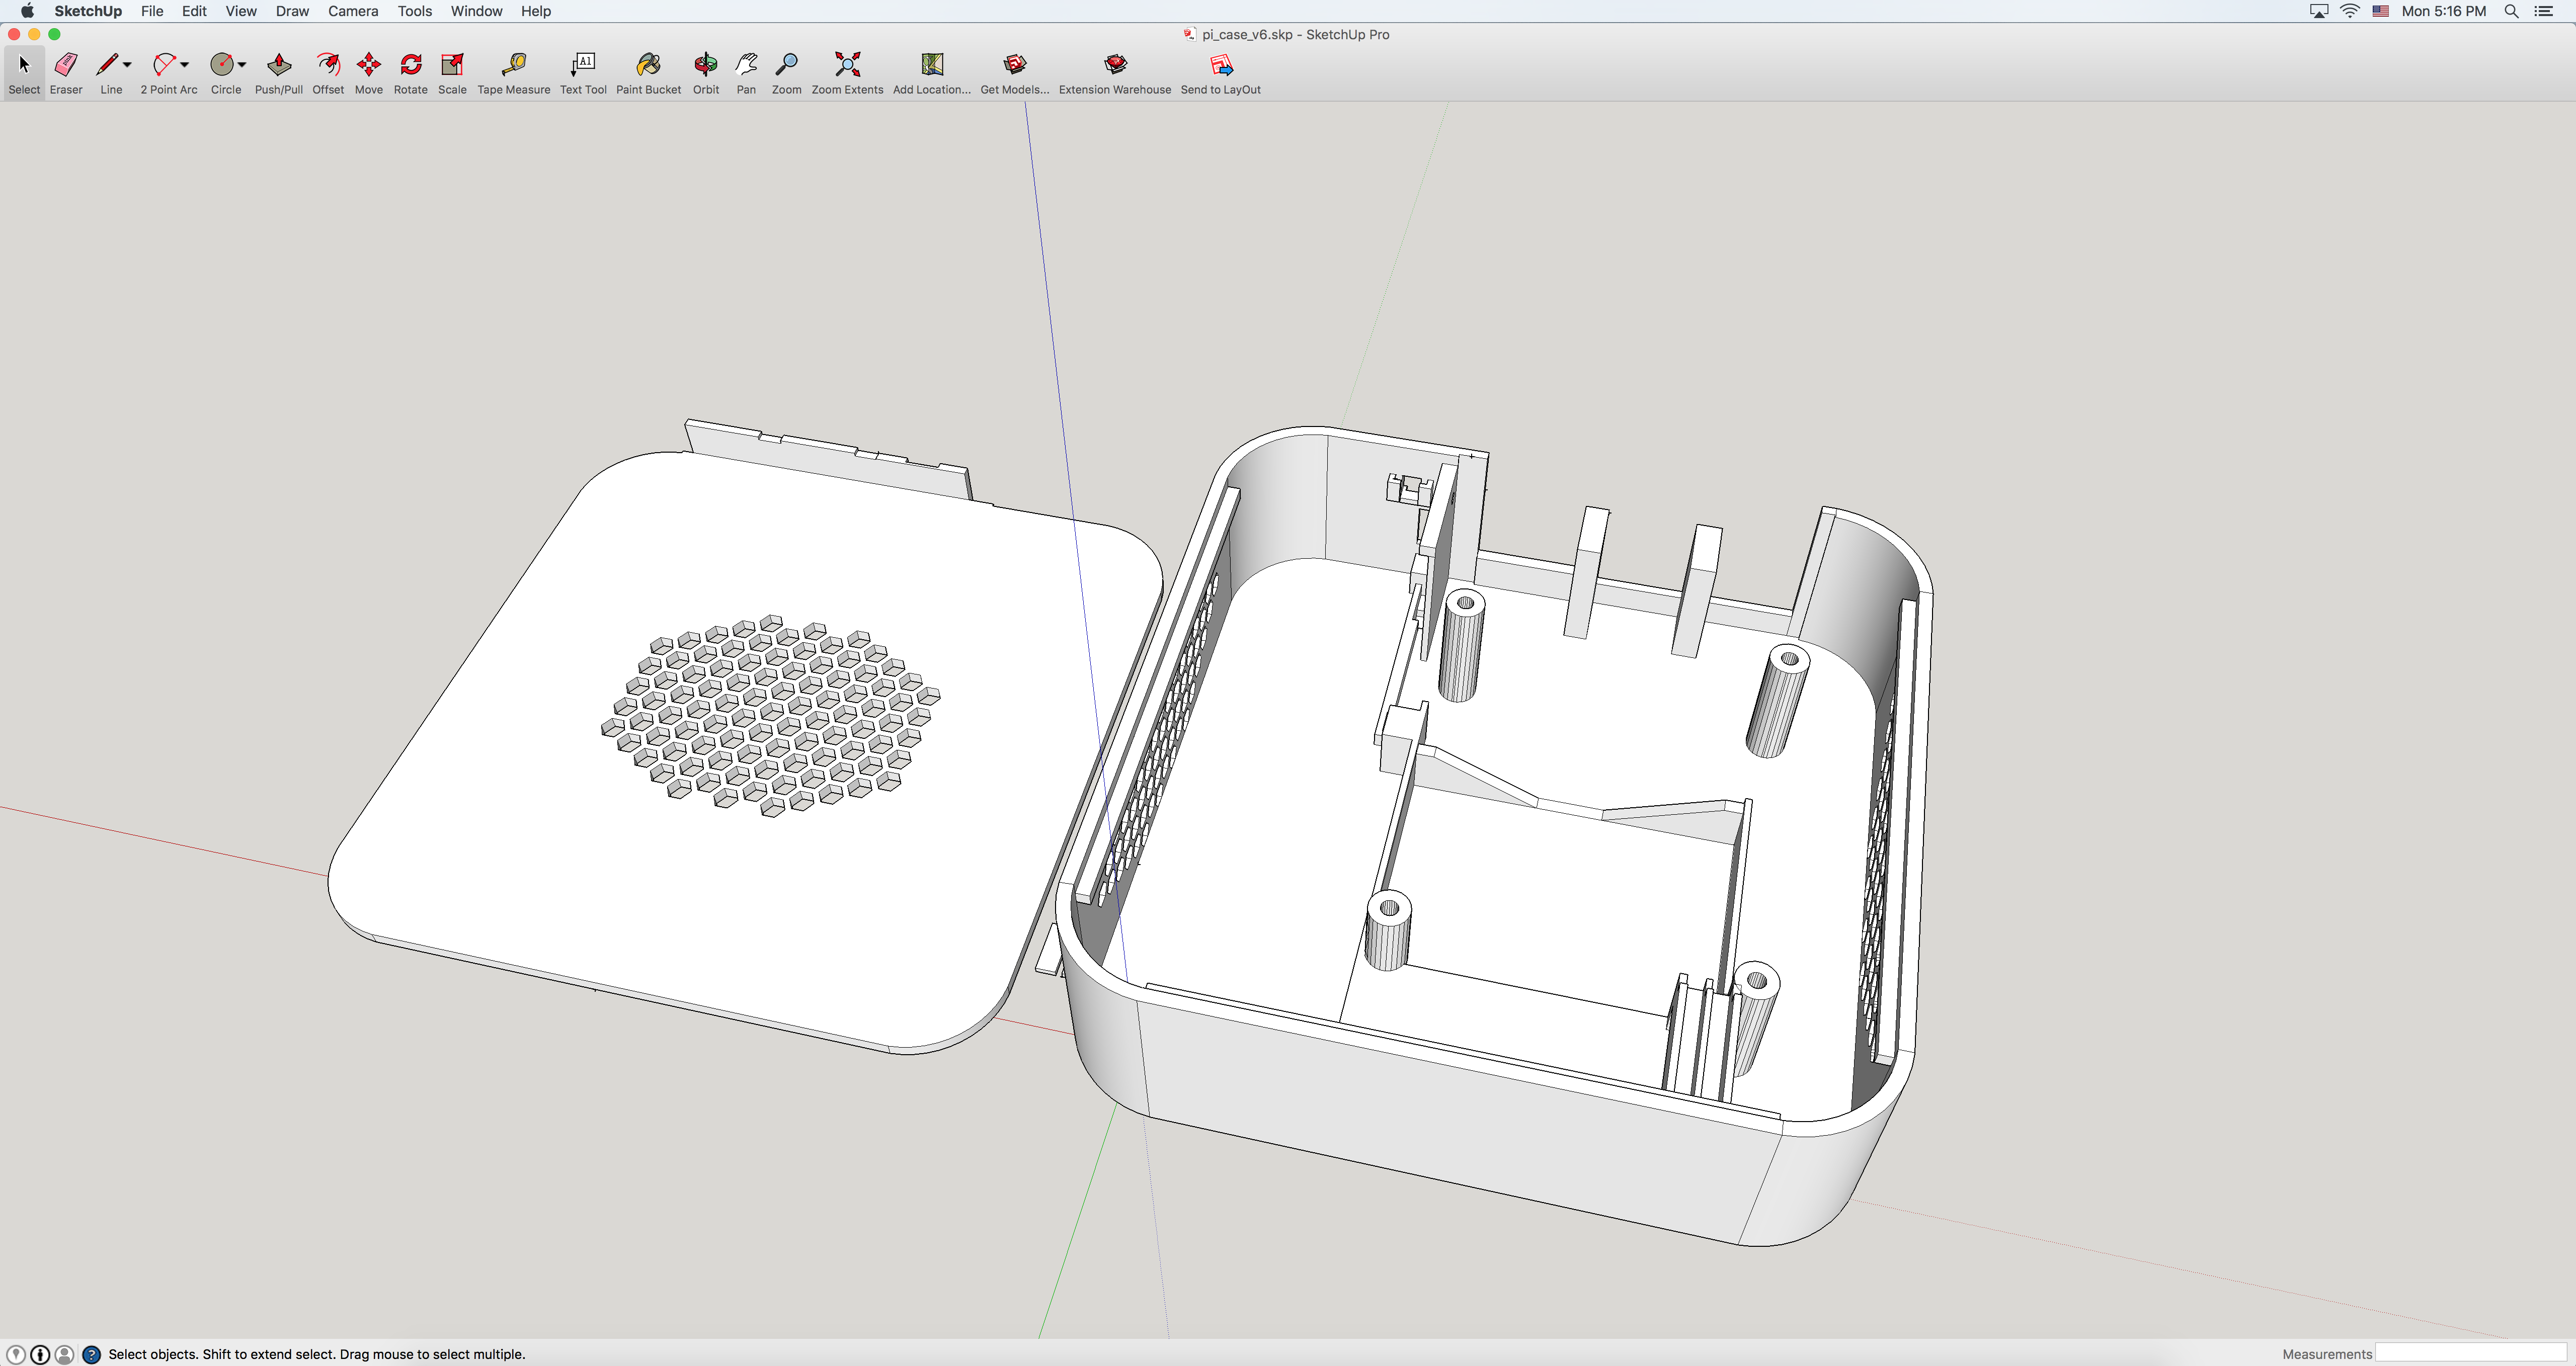
\includegraphics[width=8cm]{./images/V6.png}
		\caption{Pi Case Version5 and Version6}
	\end{figure}
\end{center}
\begin{center}
	\begin{figure}[h]
		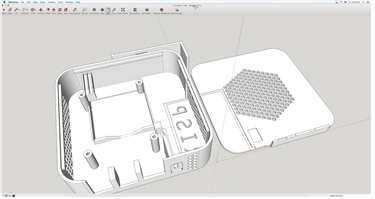
\includegraphics[width=8cm]{./images/V7.png}
		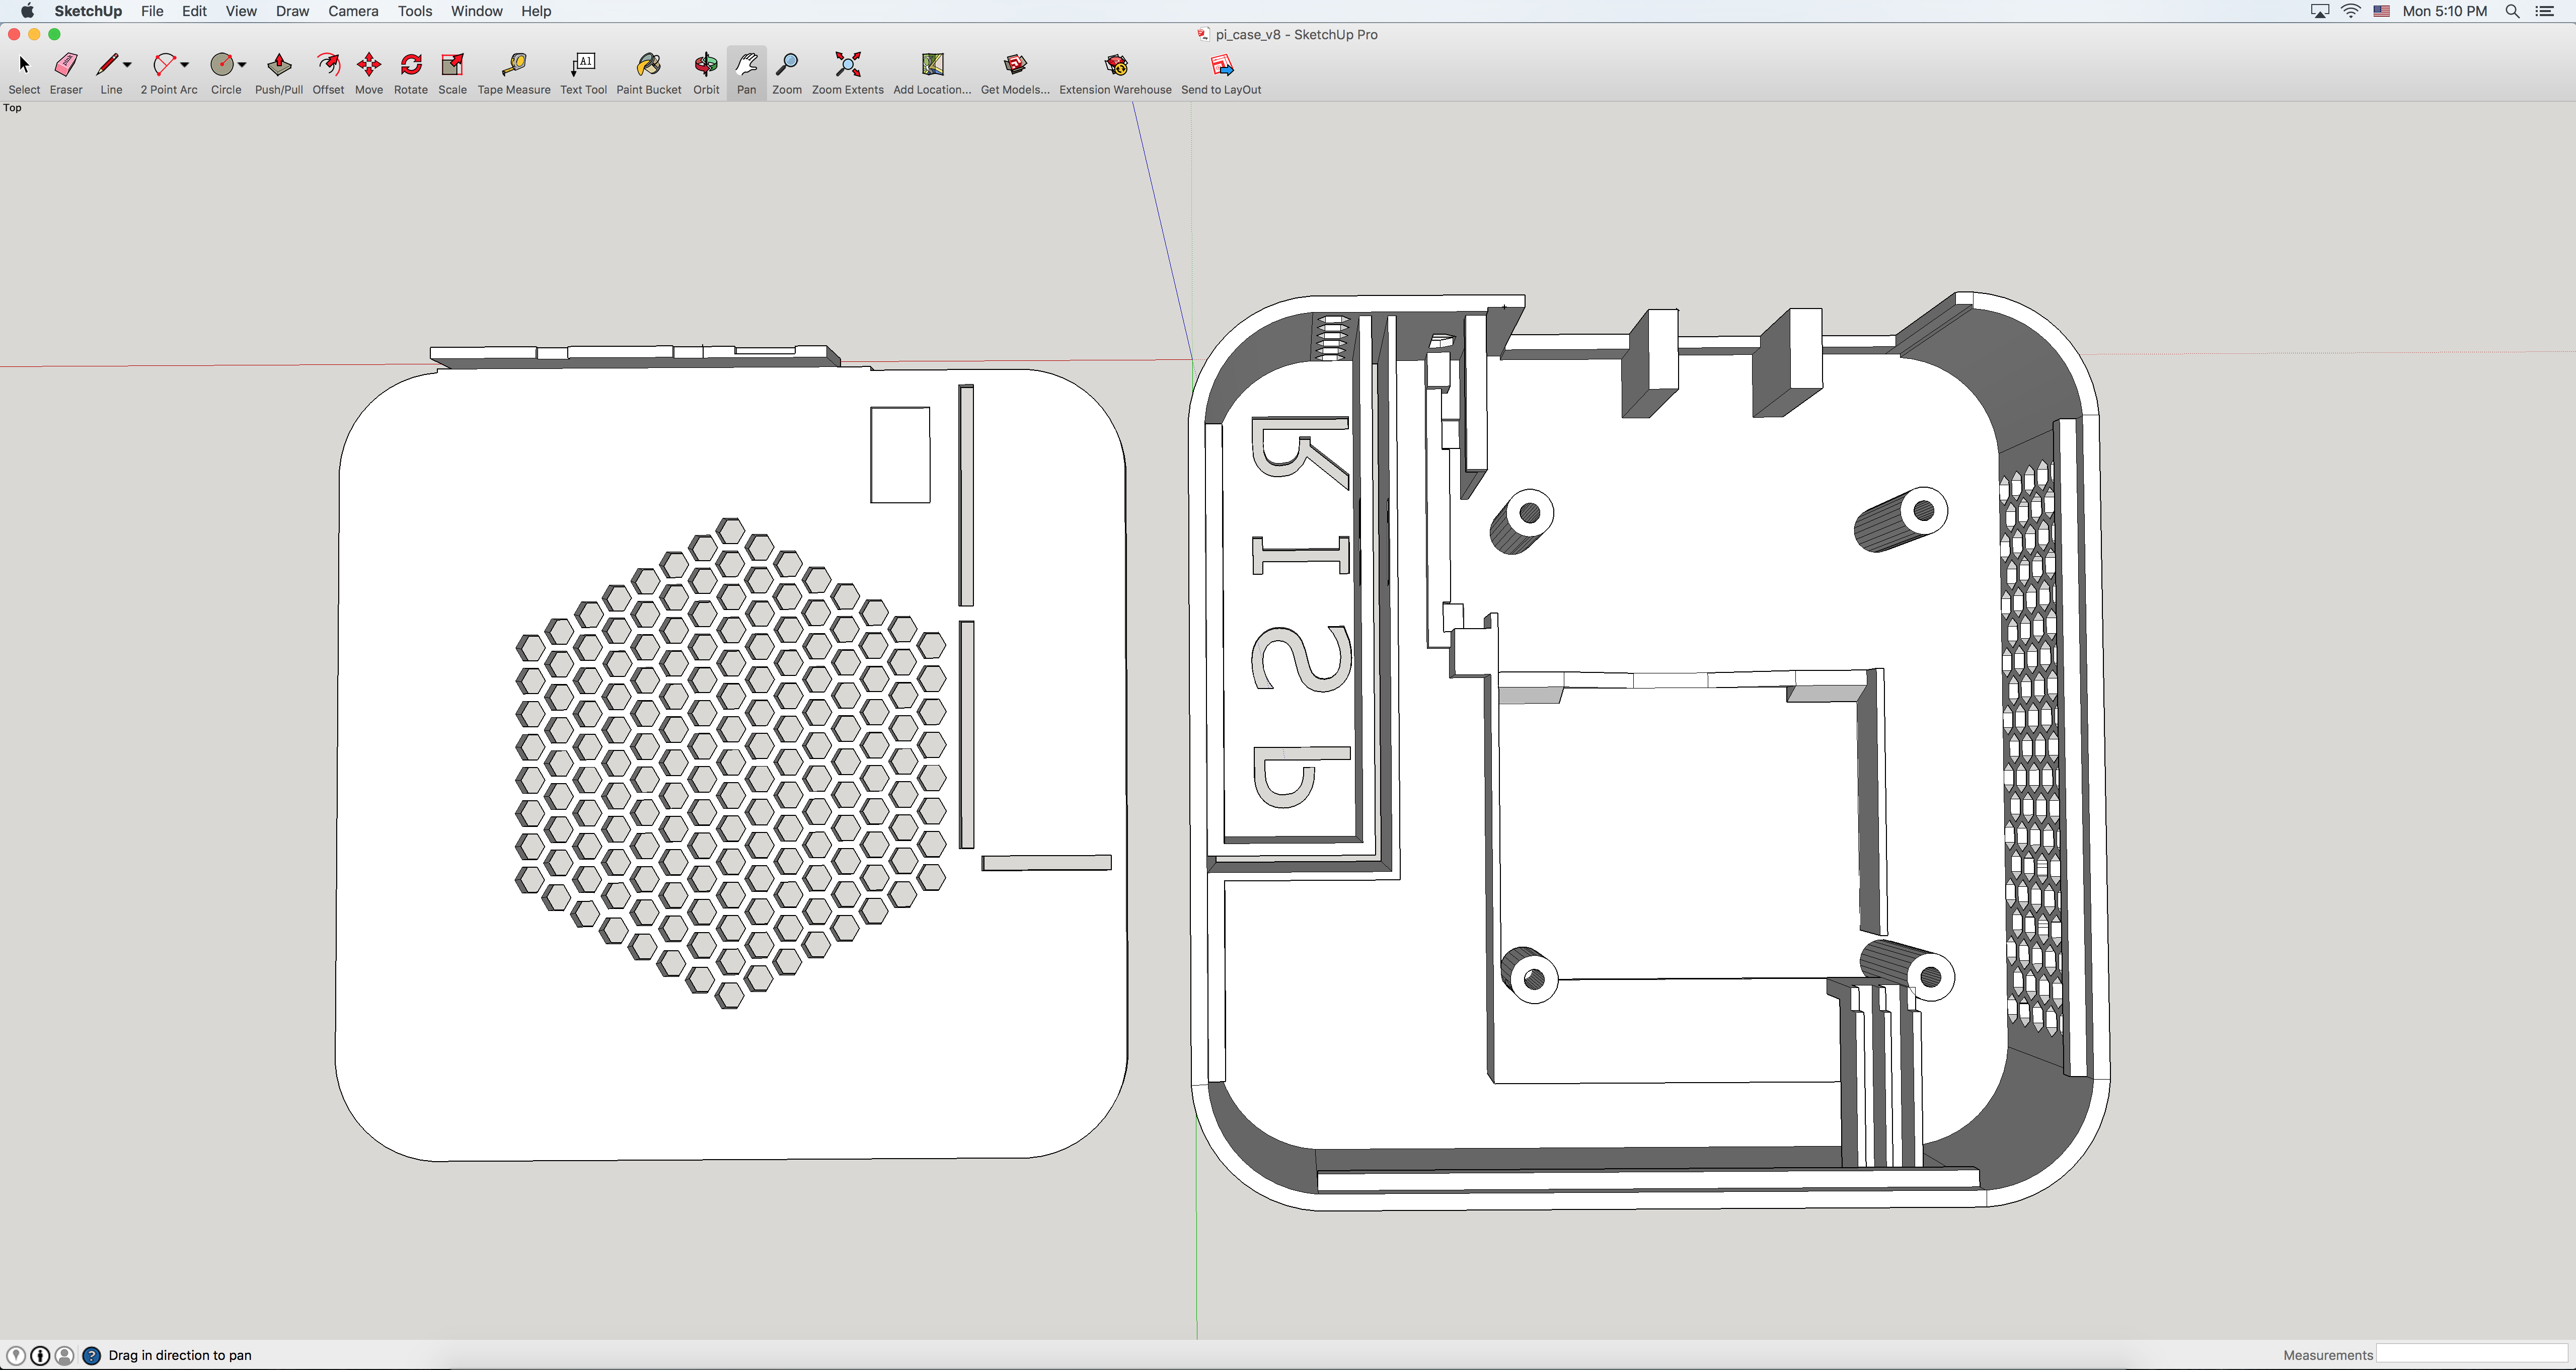
\includegraphics[width=8cm]{./images/V8.png}
		\caption{Pi Case Version7 and Version8}
	\end{figure}
\end{center}
\end{document}
